
        \documentclass[12p]{article}
        \usepackage[margin=1in, left=1.5in, includefoot]{geometry}
        \usepackage{longtable, tabu}
        \usepackage[table, dvipsnames]{xcolor}
        \usepackage{array,booktabs}
        \usepackage{color}
        \usepackage{indentfirst}
        \usepackage{graphicx}
        \usepackage{float}
        \usepackage[utf8]{inputenc}
        \usepackage{listings}
        \usepackage{url}
        \usepackage{multirow}
        \usepackage{seqsplit}
        
        \definecolor{ferrarired}{rgb}{1.0, 0.11, 0.0}
        \definecolor{orange(colorwheel)}{rgb}{1.0, 0.5, 0.0}
        \definecolor{deepskyblue}{rgb}{0.0, 0.75, 1.0}
        \definecolor{grannysmithapple}{rgb}{0.66, 0.89, 0.63}
        \definecolor{gray(x11gray)}{rgb}{0.75, 0.75, 0.75}
        \definecolor{amber}{rgb}{1.0, 0.75, 0.0}
        
        \newcommand{\icon}[1]{\includegraphics[height=12pt]{#1}}
        \newcommand{\hash}[1]{{\ttfamily\seqsplit{#1}}}

        \setlength{\arrayrulewidth}{0.3mm}
\setlength{\tabcolsep}{18pt}
\renewcommand{\arraystretch}{1.5}
\setlength{\parindent}{1em}
\begin{document}
\begin{titlepage}
\begin{center}
\line(1,0){320}\\
[0.25in]
\huge{\bfseries Android Analysis Report}
\line(1,0){320}\\
[0.5in]
\begin{figure}[H]
	\centering
	
\includegraphics[scale=0.5]{/home/miki/Documents/GITHUB/AndroidPermissions/python/vulns/report_icons/logo.png}
\end{figure}
\textsl{\LARGE Demo app}\\
\textsf{\LARGE de.number26.android}\\
[2.5in]
\end{center}
\begin{flushright}
\textbf{\large Date 2018-06-14}
\end{flushright}
\end{titlepage}
\tableofcontents
\thispagestyle{empty}
\cleardoublepage
\setcounter{page}{1}
\section{Signature}
	\begin{longtable}{p{1.5cm} p{12.5cm} }
\textbf{Owner} & \hash{CN=Javier Cuesta Gomez, OU=Number26, O=Number26, L=Berlin, ST=Berlin, C=BE}\\ 
\textbf{Issuer} & \hash{CN=Javier Cuesta Gomez, OU=Number26, O=Number26, L=Berlin, ST=Berlin, C=BE}\\ 
\textbf{Serial Number} & \hash{66a19d3f}\\ 
\textbf{MD5} & \hash{77:2D:74:B0:A9:1F:B1:2E:71:A4:57:F9:F1:F3:C7:AC}\\ 
\textbf{SHA1} & \hash{57:6D:B8:85:4F:A2:07:97:17:6D:39:55:32:A6:1C:75:9B:DC:01:D0}\\ 
\textbf{SHA256} & \hash{80:0F:89:B0:10:F9:EF:7C:B4:88:4E:D6:ED:CF:D0:BA:E5:0E:7F:48:4E:C0:75:17:FD:F6:61:D6:9D:65:0A:DD}\\ 
\textbf{Algorithm} & \hash{SHA256withRSA}\\ 
	\end{longtable}
\section{PERMISSIONS}
	\begin{longtable}{p{3cm} p{10cm} }
	\rowcolor{grannysmithapple!70} Type & List \\
Normal &  ACCESS\_NETWORK\_STATE \\ 
 &  ACCESS\_WIFI\_STATE \\ 
 &  INTERNET \\ 
 &  WAKE\_LOCK \\ 
\hline
Dangerous &  CAMERA \\ 
 &  ACCESS\_COARSE\_LOCATION \\ 
 &  ACCESS\_FINE\_LOCATION \\ 
 &  RECORD\_AUDIO \\ 
 &  READ\_EXTERNAL\_STORAGE \\ 
 &  WRITE\_EXTERNAL\_STORAGE \\ 
\hline
Overprivileged &  USE\_FINGERPRINT \\ 
 &  C \\ 
 &  READ\_CONTACTS \\ 
 &  BIND\_GET\_INSTALL\_REFERRER\_SERVICE \\ 
 &  READ\_GSERVICES \\ 
 &  BLUETOOTH \\ 
 &  MODIFY\_AUDIO\_SETTINGS \\ 
 &  BLUETOOTH\_ADMIN \\ 
 &  RECEIVE \\ 
 &  FLASHLIGHT \\ 
 &  BROADCAST\_STICKY \\ 
 &  PUSH\_MESSAGE \\ 
\hline
Underprivileged &  UPDATE\_DEVICE\_STATS \\ 
\hline
Automatically granted dangerous permissions &  WRITE\_CONTACTS \\ 
 &  GET\_ACCOUNTS \\ 
\hline
	\end{longtable}
\section{FINDINGS SUMMARY}\label{sec:summary}
\begin{figure}[H]
\centering
	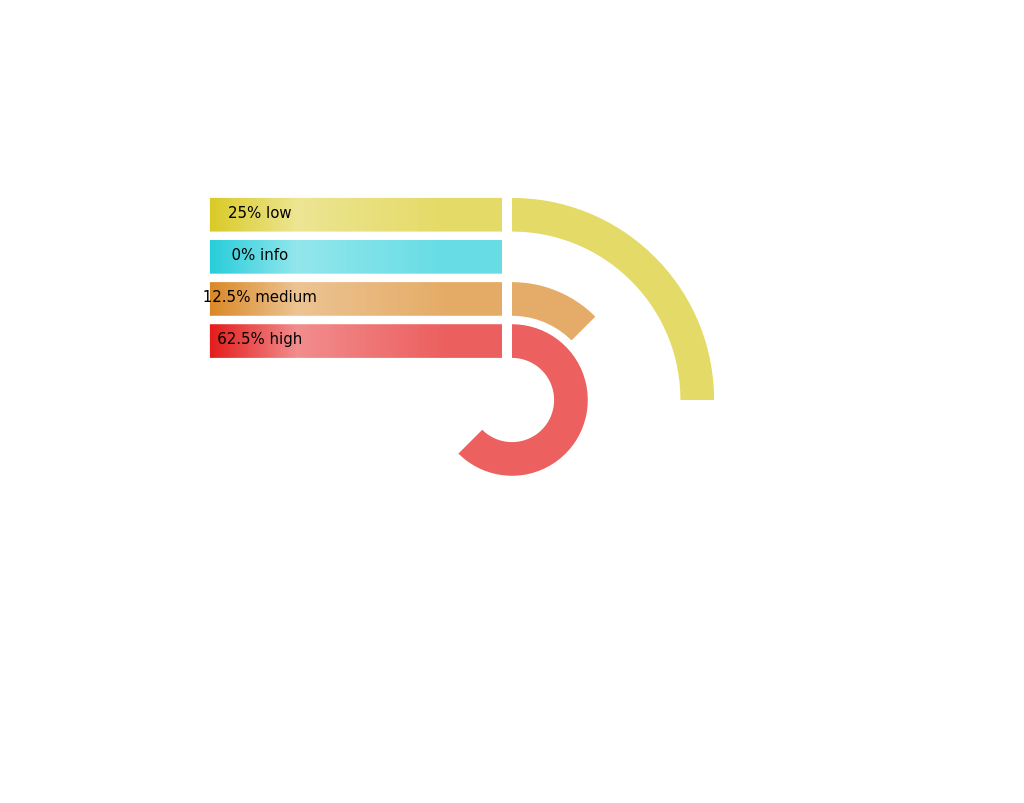
\includegraphics[scale=0.5]{/home/miki/Documents/GITHUB/AndroidPermissions/apks/playstore_apps/de_number26_android/report/pie_chart.png}
\end{figure}
	\begin{longtable}{p{0.5cm} p{10cm} p{1.5cm}}
	\rowcolor{grannysmithapple!70} Index & Title & Impact \\
	A1&Access local ressources& \color{ferrarired}\textbf{High} \\
\hline\\	A2&& \color{amber}\textbf{Low} \\
\hline\\	A3&Launch Mode of Activity \newline (de. number26. machete. android. ui. landing. SplashActivity) is not standard.& \color{ferrarired}\textbf{High} \\
\hline\\	A4&Activity \newline (de. number26. machete. android. deeplink. DeepLinkActivity) is not Protected. An intent-filter exists.& \color{ferrarired}\textbf{High} \\
\hline\\	A5&Activity \newline (de. number26. machete. android. ui. HomeActivity) is not Protected. An intent-filter exists.& \color{ferrarired}\textbf{High} \\
\hline\\	A6&Broadcast Receiver \newline (com. adjust. sdk. AdjustReferrerReceiver) is not Protected. [android:exported=true]& \color{ferrarired}\textbf{High} \\
\hline\\	A7&Service \newline (de. number26. machete. android. refactor. data. remote\_ message. reception. FirebaseMessageCapturerService) is not Protected. An intent-filter exists.& \color{ferrarired}\textbf{High} \\
\hline\\	A8&Service \newline (de. number26. machete. android. refactor. data. remote\_ message. registration. FirebaseDeviceTokenService) is not Protected. An intent-filter exists.& \color{ferrarired}\textbf{High} \\
\hline\\	A9&Launch Mode of Activity \newline (com. salesforce. android. chat. ui. internal. chatfeed. ChatFeedActivity) is not standard.& \color{ferrarired}\textbf{High} \\
\hline\\	A10&Launch Mode of Activity \newline (com. salesforce. android. chat. ui. internal. prechat. PreChatActivity) is not standard.& \color{ferrarired}\textbf{High} \\
\hline\\	A11&Service \newline (com. google. firebase. messaging. FirebaseMessagingService) is not Protected. [android:exported=true]& \color{ferrarired}\textbf{High} \\
\hline\\	A12&Service \newline (com. google. firebase. iid. FirebaseInstanceIdService) is not Protected. [android:exported=true]& \color{ferrarired}\textbf{High} \\
\hline\\	A13&Activity \newline (de. idnow. sdk. Activities\_ VideoLiveStreamActivity\_ IceLink) is not Protected. [android:exported=true]& \color{ferrarired}\textbf{High} \\
\hline\\	A14&High Intent Priority \newline (900) [android:priority]& \color{orange(colorwheel)}\textbf{Medium} \\
\hline\\	A15&High Intent Priority \newline (900) [android:priority]& \color{orange(colorwheel)}\textbf{Medium} \\
\hline\\	A16&& \color{amber}\textbf{Low} \\
\hline\\	\end{longtable}
\cleardoublepage
\newpage
\section{DETAILED FINDINGS}
\subsection{A1: Access local ressources}
\subsubsection*{\protect\icon{/home/miki/Documents/GITHUB/AndroidPermissions/python/vulns/report_icons/basic_sheet.png} Description}

\subsubsection*{\protect\icon{/home/miki/Documents/GITHUB/AndroidPermissions/python/vulns/report_icons/basic_magnifier.png} Evidence}
\path{/home/miki/Documents/GITHUB/AndroidPermissions/apks/playstore_apps/de_number26_android/app/smali/de/idnow/sdk/Activities_VideoLiveStreamActivity_Super.smali}

\subsubsection*{\protect\icon{/home/miki/Documents/GITHUB/AndroidPermissions/python/vulns/report_icons/basic_todo.png} Recommendation}

\subsection{A2: }
\subsubsection*{\protect\icon{/home/miki/Documents/GITHUB/AndroidPermissions/python/vulns/report_icons/basic_sheet.png} Description}

\subsubsection*{\protect\icon{/home/miki/Documents/GITHUB/AndroidPermissions/python/vulns/report_icons/basic_magnifier.png} Evidence}
\path{/home/miki/Documents/GITHUB/AndroidPermissions/apks/playstore_apps/de_number26_android/app/smali/android/arch/lifecycle/d$a$1.smali
Landroid/util/Log -> e(Ljava/lang/String;Ljava/lang/String;)}

\path{/home/miki/Documents/GITHUB/AndroidPermissions/apks/playstore_apps/de_number26_android/app/smali/android/arch/lifecycle/d$a$2.smali
Landroid/util/Log -> e(Ljava/lang/String;Ljava/lang/String;)}

\path{/home/miki/Documents/GITHUB/AndroidPermissions/apks/playstore_apps/de_number26_android/app/smali/android/arch/lifecycle/i.smali
Landroid/util/Log -> w(Ljava/lang/String;Ljava/lang/String;)}

\path{/home/miki/Documents/GITHUB/AndroidPermissions/apks/playstore_apps/de_number26_android/app/smali/android/support/v4/a/e.smali
Landroid/util/Log -> e(Ljava/lang/String;Ljava/lang/String;Ljava/lang/Throwable;)}

\path{/home/miki/Documents/GITHUB/AndroidPermissions/apks/playstore_apps/de_number26_android/app/smali/android/support/v4/a/e.smali
Landroid/util/Log -> w(Ljava/lang/String;Ljava/lang/String;)}

\path{/home/miki/Documents/GITHUB/AndroidPermissions/apks/playstore_apps/de_number26_android/app/smali/android/support/v4/a/b$b.smali
Landroid/util/Log -> w(Ljava/lang/String;Ljava/lang/String;)}

\path{/home/miki/Documents/GITHUB/AndroidPermissions/apks/playstore_apps/de_number26_android/app/smali/android/support/v4/a/b$b.smali
Landroid/util/Log -> w(Ljava/lang/String;Ljava/lang/String;)}

\path{/home/miki/Documents/GITHUB/AndroidPermissions/apks/playstore_apps/de_number26_android/app/smali/android/support/v4/a/h.smali
Landroid/util/Log -> e(Ljava/lang/String;Ljava/lang/String;)}

\path{/home/miki/Documents/GITHUB/AndroidPermissions/apks/playstore_apps/de_number26_android/app/smali/android/support/v4/a/f.smali
Landroid/util/Log -> e(Ljava/lang/String;Ljava/lang/String;Ljava/lang/Throwable;)}

\path{/home/miki/Documents/GITHUB/AndroidPermissions/apks/playstore_apps/de_number26_android/app/smali/android/support/v4/a/f.smali
Landroid/util/Log -> w(Ljava/lang/String;Ljava/lang/String;)}


\textit{snip}
\newline \textsl{For the full list view \path{/home/miki/Documents/GITHUB/AndroidPermissions/apks/playstore_apps/de_number26_android/report}}
\subsubsection*{\protect\icon{/home/miki/Documents/GITHUB/AndroidPermissions/python/vulns/report_icons/basic_todo.png} Recommendation}

\subsection{A3: Launch Mode of Activity (de. number26. machete. android. ui. landing. SplashActivity) is not standard.}
\subsubsection*{\protect\icon{/home/miki/Documents/GITHUB/AndroidPermissions/python/vulns/report_icons/basic_sheet.png} Description}
An Activity should not be having the launch mode attribute set to "singleTask/singleInstance" as it becomes root Activity and it is possible for other applications to read the contents of the calling Intent.
\subsubsection*{\protect\icon{/home/miki/Documents/GITHUB/AndroidPermissions/python/vulns/report_icons/basic_todo.png} Recommendation}
It is required to use the "standard" launch mode attribute when sensitive information is included in an Intent.
\subsection{A4: Activity (de. number26. machete. android. deeplink. DeepLinkActivity) is not Protected. An intent-filter exists.}
\subsubsection*{\protect\icon{/home/miki/Documents/GITHUB/AndroidPermissions/python/vulns/report_icons/basic_sheet.png} Description}
A  Activity is found to be shared with other apps on the device therefore leaving it accessible to any other application on the device. The presence of intent-filter indicates that the Activity is explicitly exported.
\subsubsection*{\protect\icon{/home/miki/Documents/GITHUB/AndroidPermissions/python/vulns/report_icons/basic_todo.png} Recommendation}
It is recommended to set the protection level to signature, so only applications signed with the same certificate can obtain the permission.
\subsection{A5: Activity (de. number26. machete. android. ui. HomeActivity) is not Protected. An intent-filter exists.}
\subsubsection*{\protect\icon{/home/miki/Documents/GITHUB/AndroidPermissions/python/vulns/report_icons/basic_sheet.png} Description}
A  Activity is found to be shared with other apps on the device therefore leaving it accessible to any other application on the device. The presence of intent-filter indicates that the Activity is explicitly exported.
\subsubsection*{\protect\icon{/home/miki/Documents/GITHUB/AndroidPermissions/python/vulns/report_icons/basic_todo.png} Recommendation}
It is recommended to set the protection level to signature, so only applications signed with the same certificate can obtain the permission.
\subsection{A6: Broadcast Receiver (com. adjust. sdk. AdjustReferrerReceiver) is not Protected. [android:exported=true]}
\subsubsection*{\protect\icon{/home/miki/Documents/GITHUB/AndroidPermissions/python/vulns/report_icons/basic_sheet.png} Description}
A Broadcast Receiver is found to be shared with other apps on the device therefore leaving it accessible to any other application on the device.
\subsubsection*{\protect\icon{/home/miki/Documents/GITHUB/AndroidPermissions/python/vulns/report_icons/basic_todo.png} Recommendation}
It is recommended to set the protection level to signature, so only applications signed with the same certificate can obtain the permission.
\subsection{A7: Service (de. number26. machete. android. refactor. data. remote\_ message. reception. FirebaseMessageCapturerService) is not Protected. An intent-filter exists.}
\subsubsection*{\protect\icon{/home/miki/Documents/GITHUB/AndroidPermissions/python/vulns/report_icons/basic_sheet.png} Description}
A  Service is found to be shared with other apps on the device therefore leaving it accessible to any other application on the device. The presence of intent-filter indicates that the Service is explicitly exported.
\subsubsection*{\protect\icon{/home/miki/Documents/GITHUB/AndroidPermissions/python/vulns/report_icons/basic_todo.png} Recommendation}
It is recommended to set the protection level to signature, so only applications signed with the same certificate can obtain the permission.
\subsection{A8: Service (de. number26. machete. android. refactor. data. remote\_ message. registration. FirebaseDeviceTokenService) is not Protected. An intent-filter exists.}
\subsubsection*{\protect\icon{/home/miki/Documents/GITHUB/AndroidPermissions/python/vulns/report_icons/basic_sheet.png} Description}
A  Service is found to be shared with other apps on the device therefore leaving it accessible to any other application on the device. The presence of intent-filter indicates that the Service is explicitly exported.
\subsubsection*{\protect\icon{/home/miki/Documents/GITHUB/AndroidPermissions/python/vulns/report_icons/basic_todo.png} Recommendation}
It is recommended to set the protection level to signature, so only applications signed with the same certificate can obtain the permission.
\subsection{A9: Launch Mode of Activity (com. salesforce. android. chat. ui. internal. chatfeed. ChatFeedActivity) is not standard.}
\subsubsection*{\protect\icon{/home/miki/Documents/GITHUB/AndroidPermissions/python/vulns/report_icons/basic_sheet.png} Description}
An Activity should not be having the launch mode attribute set to "singleTask/singleInstance" as it becomes root Activity and it is possible for other applications to read the contents of the calling Intent.
\subsubsection*{\protect\icon{/home/miki/Documents/GITHUB/AndroidPermissions/python/vulns/report_icons/basic_todo.png} Recommendation}
It is required to use the "standard" launch mode attribute when sensitive information is included in an Intent.
\subsection{A10: Launch Mode of Activity (com. salesforce. android. chat. ui. internal. prechat. PreChatActivity) is not standard.}
\subsubsection*{\protect\icon{/home/miki/Documents/GITHUB/AndroidPermissions/python/vulns/report_icons/basic_sheet.png} Description}
An Activity should not be having the launch mode attribute set to "singleTask/singleInstance" as it becomes root Activity and it is possible for other applications to read the contents of the calling Intent.
\subsubsection*{\protect\icon{/home/miki/Documents/GITHUB/AndroidPermissions/python/vulns/report_icons/basic_todo.png} Recommendation}
It is required to use the "standard" launch mode attribute when sensitive information is included in an Intent.
\subsection{A11: Service (com. google. firebase. messaging. FirebaseMessagingService) is not Protected. [android:exported=true]}
\subsubsection*{\protect\icon{/home/miki/Documents/GITHUB/AndroidPermissions/python/vulns/report_icons/basic_sheet.png} Description}
A Service is found to be shared with other apps on the device therefore leaving it accessible to any other application on the device.
\subsubsection*{\protect\icon{/home/miki/Documents/GITHUB/AndroidPermissions/python/vulns/report_icons/basic_todo.png} Recommendation}
It is recommended to set the protection level to signature, so only applications signed with the same certificate can obtain the permission.
\subsection{A12: Service (com. google. firebase. iid. FirebaseInstanceIdService) is not Protected. [android:exported=true]}
\subsubsection*{\protect\icon{/home/miki/Documents/GITHUB/AndroidPermissions/python/vulns/report_icons/basic_sheet.png} Description}
A Service is found to be shared with other apps on the device therefore leaving it accessible to any other application on the device.
\subsubsection*{\protect\icon{/home/miki/Documents/GITHUB/AndroidPermissions/python/vulns/report_icons/basic_todo.png} Recommendation}
It is recommended to set the protection level to signature, so only applications signed with the same certificate can obtain the permission.
\subsection{A13: Activity (de. idnow. sdk. Activities\_ VideoLiveStreamActivity\_ IceLink) is not Protected. [android:exported=true]}
\subsubsection*{\protect\icon{/home/miki/Documents/GITHUB/AndroidPermissions/python/vulns/report_icons/basic_sheet.png} Description}
A Activity is found to be shared with other apps on the device therefore leaving it accessible to any other application on the device.
\subsubsection*{\protect\icon{/home/miki/Documents/GITHUB/AndroidPermissions/python/vulns/report_icons/basic_todo.png} Recommendation}
It is recommended to set the protection level to signature, so only applications signed with the same certificate can obtain the permission.
\subsection{A14: High Intent Priority (900) [android:priority]}
\subsubsection*{\protect\icon{/home/miki/Documents/GITHUB/AndroidPermissions/python/vulns/report_icons/basic_sheet.png} Description}
By setting an intent priority higher than another intent, the app effectively overrides other requests.
\subsubsection*{\protect\icon{/home/miki/Documents/GITHUB/AndroidPermissions/python/vulns/report_icons/basic_todo.png} Recommendation}
If possible, do not set higher priorities for specific intents in the manifest file.
\subsection{A15: High Intent Priority (900) [android:priority]}
\subsubsection*{\protect\icon{/home/miki/Documents/GITHUB/AndroidPermissions/python/vulns/report_icons/basic_sheet.png} Description}
By setting an intent priority higher than another intent, the app effectively overrides other requests.
\subsubsection*{\protect\icon{/home/miki/Documents/GITHUB/AndroidPermissions/python/vulns/report_icons/basic_todo.png} Recommendation}
If possible, do not set higher priorities for specific intents in the manifest file.
\subsection{A16: }
\subsubsection*{\protect\icon{/home/miki/Documents/GITHUB/AndroidPermissions/python/vulns/report_icons/basic_sheet.png} Description}

\subsubsection*{\protect\icon{/home/miki/Documents/GITHUB/AndroidPermissions/python/vulns/report_icons/basic_magnifier.png} Evidence}
\path{/home/miki/Documents/GITHUB/AndroidPermissions/apks/playstore_apps/de_number26_android/app/smali/android/arch/lifecycle/k.smali forName}

\path{/home/miki/Documents/GITHUB/AndroidPermissions/apks/playstore_apps/de_number26_android/app/smali/android/arch/lifecycle/k.smali getSuperclass}

\path{/home/miki/Documents/GITHUB/AndroidPermissions/apks/playstore_apps/de_number26_android/app/smali/android/arch/lifecycle/a$b.smali invoke}

\path{/home/miki/Documents/GITHUB/AndroidPermissions/apks/playstore_apps/de_number26_android/app/smali/android/arch/lifecycle/a.smali getSuperclass}

\path{/home/miki/Documents/GITHUB/AndroidPermissions/apks/playstore_apps/de_number26_android/app/smali/android/support/v4/a/e.smali forName}

\path{/home/miki/Documents/GITHUB/AndroidPermissions/apks/playstore_apps/de_number26_android/app/smali/android/support/v4/a/e.smali invoke}

\path{/home/miki/Documents/GITHUB/AndroidPermissions/apks/playstore_apps/de_number26_android/app/smali/android/support/v4/a/e.smali invoke}

\path{/home/miki/Documents/GITHUB/AndroidPermissions/apks/playstore_apps/de_number26_android/app/smali/android/support/v4/a/f.smali forName}

\path{/home/miki/Documents/GITHUB/AndroidPermissions/apks/playstore_apps/de_number26_android/app/smali/android/support/v4/a/f.smali invoke}

\path{/home/miki/Documents/GITHUB/AndroidPermissions/apks/playstore_apps/de_number26_android/app/smali/android/support/v4/a/f.smali invoke}


\textit{snip}
\newline \textsl{For the full list view \path{/home/miki/Documents/GITHUB/AndroidPermissions/apks/playstore_apps/de_number26_android/report}}
\subsubsection*{\protect\icon{/home/miki/Documents/GITHUB/AndroidPermissions/python/vulns/report_icons/basic_todo.png} Recommendation}

\cleardoublepage
\newpage
\section{VISUALIZATIONS}
\subsection{Chord Diagram - Class Relations}
\begin{figure}[H]
	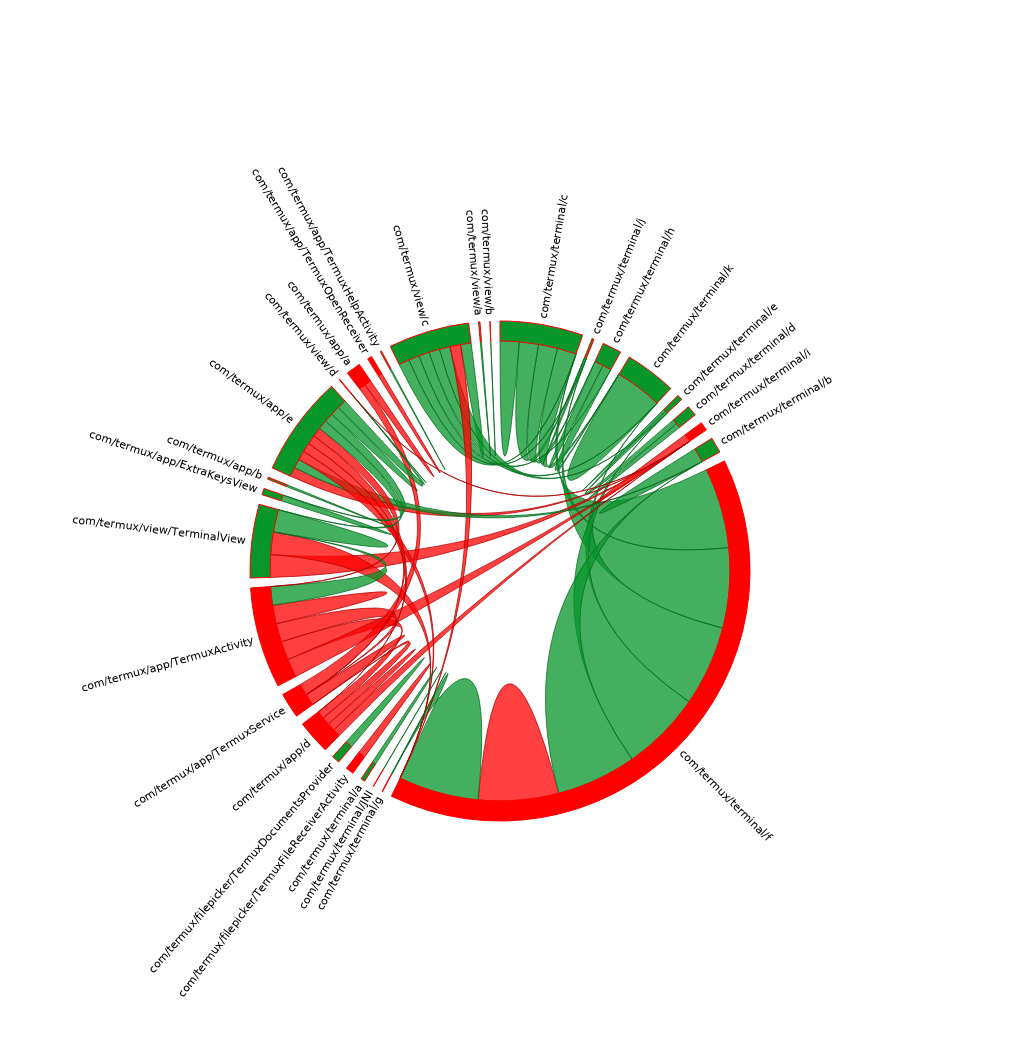
\includegraphics[scale=0.45]{/home/miki/Documents/GITHUB/AndroidPermissions/apks/playstore_apps/de_number26_android/report/chord_diagram.png}\end{figure}\subsection{Hot Spot - System Overview}
\begin{figure}[H]
\centering
	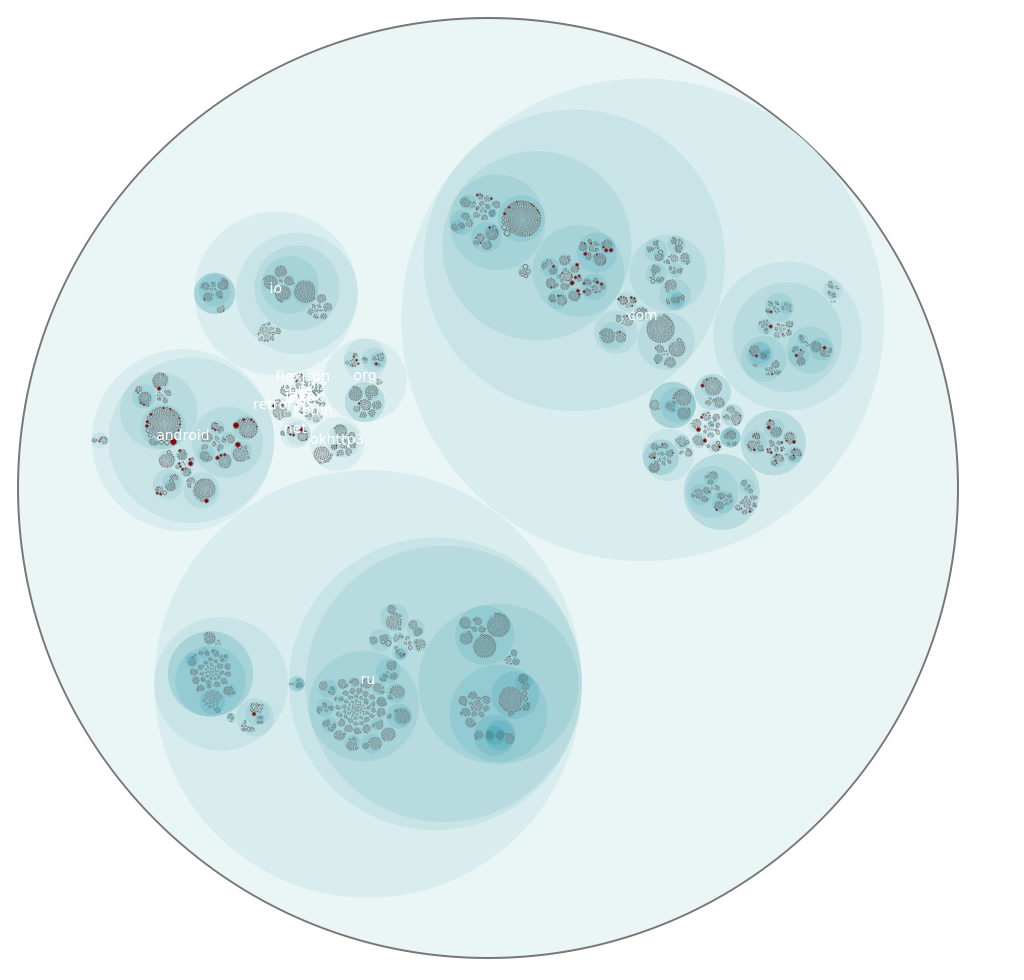
\includegraphics[scale=0.5]{/home/miki/Documents/GITHUB/AndroidPermissions/apks/playstore_apps/de_number26_android/report/hotspot.png}\end{figure}\begin{longtable}{p{0.3cm} p{12cm}}
\rowcolor{orange} Index & Class \\
1 & \path{/home/miki/Documents/GITHUB/AndroidPermissions/apks/playstore_apps/de_number26_android/app/smali/com/adjust/sdk/ActivityHandler.smali} \\
2 & \path{/home/miki/Documents/GITHUB/AndroidPermissions/apks/playstore_apps/de_number26_android/app/smali/de/idnow/sdk/Activities_VideoLiveStreamActivity_IceLink.smali} \\
3 & \path{/home/miki/Documents/GITHUB/AndroidPermissions/apks/playstore_apps/de_number26_android/app/smali/com/opentok/android/Session.smali} \\
4 & \path{/home/miki/Documents/GITHUB/AndroidPermissions/apks/playstore_apps/de_number26_android/app/smali/com/adjust/sdk/InstallReferrer.smali} \\
5 & \path{/home/miki/Documents/GITHUB/AndroidPermissions/apks/playstore_apps/de_number26_android/app/smali/de/idnow/sdk/Network_OkHttpWebSocket.smali} \\
6 & \path{/home/miki/Documents/GITHUB/AndroidPermissions/apks/playstore_apps/de_number26_android/app/smali/de/idnow/sdk/Activities_VideoLiveStreamActivity_Super.smali} \\
7 & \path{/home/miki/Documents/GITHUB/AndroidPermissions/apks/playstore_apps/de_number26_android/app/smali/android/support/multidex/a.smali} \\
8 & \path{/home/miki/Documents/GITHUB/AndroidPermissions/apks/playstore_apps/de_number26_android/app/smali/android/support/multidex/b.smali} \\
9 & \path{/home/miki/Documents/GITHUB/AndroidPermissions/apks/playstore_apps/de_number26_android/app/smali/com/adjust/sdk/Util.smali} \\
10 & \path{/home/miki/Documents/GITHUB/AndroidPermissions/apks/playstore_apps/de_number26_android/app/smali/com/google/android/gms/internal/zzdvj.smali} \\
	\end{longtable}
\end{document}
